%=============================================================
% CHAPTER 1: INTRODUCTION
%=============================================================

This thesis is submitted in partial fulfillment of the requirements for the degree of
\textit{[Degree Name]} at the \textit{Alma Mater Studiorum -- Università di Bologna}.
The work presented herein investigates \textit{[brief one-line description of the topic]},
with the aim of contributing meaningful insights to the field of \textit{[Research Field]}.
As noted by Lamport~\cite{lamport1994latex}, the use of structured document preparation
systems greatly enhances the clarity and reproducibility of academic writing.

The remainder of this chapter is organized as follows: Section~\ref{sec:background}
provides the background and motivation, Section~\ref{sec:problem} defines the problem
statement, Section~\ref{sec:objectives} outlines the research objectives,
Section~\ref{sec:methodology} briefly describes the methodology, and
Section~\ref{sec:outline} presents the overall structure of the thesis.

%-------------------------------------------------------------
\section{Background and Motivation}
\label{sec:background}
%-------------------------------------------------------------

\subsection{Historical Context}
\label{subsec:historical}

The study of \textit{[topic]} has evolved significantly over the past decades.
Early contributions by Knuth~\cite{knuth1984texbook} laid the foundational
principles of typesetting that continue to inform modern academic publishing.
The \textit{Università di Bologna}, founded circa 1088 and widely regarded as
the world's oldest university in continuous operation~\cite{rashdall1936universities},
has long been at the forefront of advances in \textit{[field]}, making it a
fitting home for the present work.

The rapid growth of digital communication and open-access publishing has further
underscored the importance of standardized document formats~\cite{mittelbach2004latex}.
In this context, reproducible and well-structured academic templates serve not
only an aesthetic purpose but also a functional one, enabling consistent
dissemination of scholarly output~\cite{knuth1984texbook}.

\subsection{Current State of the Art}
\label{subsec:stateofart}

Recent developments in \textit{[field]} have demonstrated the growing importance
of \textit{[specific topic]}. Influential surveys such as~\cite{survey2020field}
have shown that \textit{[key finding or trend]}. Meanwhile, seminal works
by~\cite{author_method2019} proposed novel approaches that addressed several
long-standing limitations in the area. Despite these advances, several
open challenges remain, particularly in the areas of:

\begin{itemize}
    \item \textbf{Challenge 1:} As identified by~\cite{challenge_paper2021},
          a brief description of the first limitation or gap.
    \item \textbf{Challenge 2:} A brief description of the second limitation,
          further discussed in~\cite{mittelbach2004latex}.
    \item \textbf{Challenge 3:} A brief description of the third limitation or gap.
\end{itemize}

\begin{figure}[htbp]
\centering
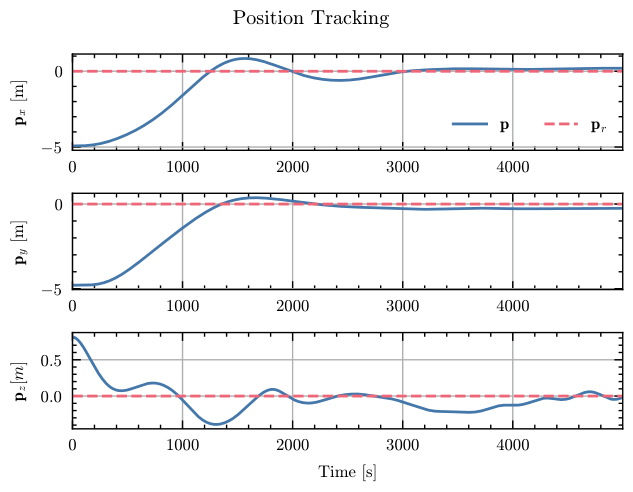
\includegraphics[width=0.75\textwidth]{figs/pos_pos.png}
\caption{An Exmaple on publishing the Images}
\label{fig:pos_tracking}
\end{figure}

These gaps collectively motivate the research presented in this thesis.

%-------------------------------------------------------------
\section{Problem Statement}
\label{sec:problem}
%-------------------------------------------------------------

\subsection{Definition of the Problem}
\label{subsec:problem-def}

The central problem addressed in this thesis can be formally stated as follows:

\begin{quote}
    \textit{``Given [input/context], how can one [action/method] in order to
    achieve [desired outcome], while satisfying [constraints or requirements]?''}
\end{quote}

This problem is significant because, as argued by~\cite{problemref2018},
\textit{[explain why it matters in theory and/or practice]}. Without an adequate
solution, \textit{[describe the consequences or limitations that persist]},
a concern echoed in the broader literature~\cite{survey2020field}.

\subsection{Scope and Limitations}
\label{subsec:scope}

While the problem domain is broad, this thesis focuses specifically on
\textit{[narrowed scope]}, in line with the methodology suggested
by~\cite{researchmethod2017}. The following boundaries are explicitly defined
for the purposes of this work:

\begin{enumerate}
    \item The analysis is confined to \textit{[domain/dataset/environment]}.
    \item Interactions with \textit{[excluded factor]} are not considered,
          following the assumptions of~\cite{author_method2019}.
    \item Results are validated under \textit{[specific experimental conditions]}.
\end{enumerate}

%-------------------------------------------------------------
\section{Research Objectives}
\label{sec:objectives}
%-------------------------------------------------------------

\subsection{Primary Objectives}
\label{subsec:primary-obj}

Drawing from the gaps identified in~\cite{survey2020field}
and~\cite{challenge_paper2021}, the primary objectives of this thesis are:

\begin{enumerate}
    \item To \textit{[first main goal]} by means of \textit{[approach]}.
    \item To \textit{[second main goal]} through the application of \textit{[method]},
          inspired by the framework of~\cite{author_method2019}.
    \item To \textit{[third main goal]} with respect to \textit{[criterion]}.
\end{enumerate}

\subsection{Secondary Objectives}
\label{subsec:secondary-obj}

In addition to the primary objectives, this work also aims to:

\begin{itemize}
    \item Provide a reusable \textit{[artifact, tool, or framework]} for
          future research in the field, following best practices outlined
          in~\cite{researchmethod2017}.
    \item Contribute to the existing literature by \textit{[type of contribution]}.
    \item Establish a benchmark for evaluating \textit{[aspect]} under
          \textit{[conditions]}, complementing the evaluation protocols
          of~\cite{challenge_paper2021}.
\end{itemize}

%-------------------------------------------------------------
\section{Research Methodology}
\label{sec:methodology}
%-------------------------------------------------------------

\subsection{Overall Approach}
\label{subsec:approach}

This research adopts a \textit{[qualitative / quantitative / mixed]} methodology,
consistent with established practices in the field~\cite{researchmethod2017}.
The work is structured around three main phases:

\begin{enumerate}
    \item \textbf{Phase 1 -- Literature Review:} A systematic review of existing
          work is conducted following the guidelines of~\cite{survey2020field},
          to identify relevant theories, methods, and open problems.
    \item \textbf{Phase 2 -- Design and Implementation:} Based on the findings
          of the review, a \textit{[model/system/framework]} is designed and
          implemented, drawing on principles from~\cite{author_method2019}.
    \item \textbf{Phase 3 -- Evaluation:} The proposed solution is evaluated
          using \textit{[metrics/datasets/experiments]}, and results are compared
          against the baselines established in~\cite{problemref2018}.
\end{enumerate}

\begin{table}[h]
\centering
\caption{Example of Table}
\label{tab:robot_params}
\begin{tabular}{lll}
\hline
Parameter & Symbol & Value \\
\hline
Mass & $m$ & 2.0 kg \\
Inertia & $J$ & $0.062$ kg$\cdot$m$^2$ \\
Arm length & $l$ & 0.39 m \\

\hline
\end{tabular}
\end{table}


\subsection{Tools and Technologies}
\label{subsec:tools}

The document itself is typeset using \LaTeX~\cite{lamport1994latex}, with
package management and compilation handled via the \texttt{latexmk} build
system~\cite{mittelbach2004latex}. The following tools are also employed:

\begin{itemize}
    \item \textbf{Programming Language:} \textit{[e.g., Python 3.10]}
    \item \textbf{Frameworks:} \textit{[e.g., TensorFlow, PyTorch, scikit-learn]}
    \item \textbf{Hardware:} \textit{[e.g., GPU cluster, local workstation specs]}
    \item \textbf{Version Control:} \textit{[e.g., Git / GitHub]}
\end{itemize}

%-------------------------------------------------------------
\section{Contributions}
\label{sec:contributions}
%-------------------------------------------------------------

The main contributions of this thesis, which extend the work
of~\cite{author_method2019} and~\cite{challenge_paper2021}, can be
summarized as follows:

\begin{enumerate}
    \item \textbf{Contribution 1:} \textit{[Describe the first novel contribution
          clearly and concisely.]}
    \item \textbf{Contribution 2:} \textit{[Describe the second novel contribution,
          e.g., a new algorithm, dataset, or theoretical result.]}
    \item \textbf{Contribution 3:} \textit{[Describe any additional contributions,
          such as open-source code, empirical findings, or design guidelines.]}
\end{enumerate}

Parts of this work have been published in / submitted to
\textit{[Conference/Journal Name, Year]}~\cite{ownpaper}.

%-------------------------------------------------------------
\section{Thesis Outline}
\label{sec:outline}
%-------------------------------------------------------------

The remainder of this thesis is structured as follows:

\begin{description}
    \item[\textbf{Chapter~\ref{chap:relatedwork}} -- Related Work:]
        Reviews the relevant literature and theoretical foundations,
        building upon the surveys of~\cite{survey2020field}.

    \item[\textbf{Chapter~\ref{chap:methodology}} -- Methodology:]
        Presents the proposed approach, detailing the design decisions,
        algorithms, and implementation choices inspired by~\cite{author_method2019}.

    \item[\textbf{Chapter~\ref{chap:results}} -- Results and Discussion:]
        Reports the experimental setup, results, and a critical analysis
        of the findings, benchmarked against~\cite{problemref2018}.

    \item[\textbf{Chapter~\ref{chap:conclusion}} -- Conclusion:]
        Summarizes the key findings, reflects on the limitations of the
        work, and suggests directions for future research.
\end{description}